\chapter{レーザ波長および受信波長構成の最適条件の検討}\label{chapt2}

本章では, ラマンDIALによる二酸化硫黄分布観測を対象として,
統計誤差および干渉誤差の波長依存性を数値シミュレーションにより評価し,
レーザ波長および受信波長構成の最適条件について検討した. 

\section{ラマンDIALの統計誤差}
ラマンDIALによる測定で発生する統計誤差は
\cref{equ:stat_err}で求められる\cite{StatErrorEqu}. 
式中の$D$はダークカウント, $B_j$は背景光雑音, 
$F$はディテクターの雑音指数を表す. 
$\mathrm{i}=1,2$ はon波長及びoff波長,  
$\mathrm{j}=1,2$ は視線距離$R_1, R_2$に相当する. 
\begin{align}
    \staterr 
    &= \dfrac{1}{2\Delta\subrm{\sigma}{SO2} \Delta R}\ab[
        \sum^2_{i=1}\sum^2_{j=1}
        \frac{D+(P_{ij}+B_j)F}{P_{ij}}
    ]^{1/2}
    \label{equ:stat_err}
\end{align}

\cref{equ:stat_err}より, 
統計誤差\staterr はレーザ波長$\subrm{\lambda}{ls}$に依存し, 
依存関係は\cref{fig:staterr_dep}に表せる. 

\begin{figure}
\centering
\begin{tikzpicture}[
    mynode/.style={
        draw, 
        rectangle, 
        rounded corners, 
        minimum width=4cm, 
        minimum height=1cm,
        align=center
    }
]
    % 各段のY座標（等間隔）
    \def\first{0}      % 1段目：レーザ波長
    \def\second{-2}     % 2段目：ラマン散乱波長
    \def\third{-4}     % 3段目：PとΔσ
    \def\fourth{-6}     % 4段目：統計誤差

    % ノード定義
    \node[mynode, fill=blue!15] (lambda_ls) at (0,\first) {レーザ波長 $\subrm{\lambda}{ls}$};
    \node[mynode] (lambda_ram) at (0,\second) {ラマン散乱波長 $\subrm{\lambda}{ram}$};
    \node[mynode] (P) at (-3,\third) {受信光子数 $P$};
    \node[mynode] (dxs) at (3,\third) {\ce{SO2}差分吸収断面積 $\Delta\subrm{\sigma}{SO2}$};
    \node[mynode, fill=red!20] (staterr) at (0,\fourth) {統計誤差 $\staterr$};

    % 矢印
    \draw[->, thick] (lambda_ram) -- (lambda_ls) node[midway, left] {依存};
    \draw[->, thick] (P) -- (lambda_ram);
    \draw[->, thick] (dxs) -- (lambda_ram);
    \draw[->, thick] (staterr) -- (P);
    \draw[->, thick] (staterr) -- (dxs);
\end{tikzpicture}
\caption{ラマンDIALにおけるレーザ波長$\subrm{\lambda}{ls}$と統計誤差 $\staterr$ の依存関係}
\label{fig:staterr_dep}
\end{figure}

\noindent
\ce{SO2}吸収が強すぎる
ラマン散乱波長$\subrm{\lambda}{ram}$
で$P$は小さくなる一方で, 
\ce{SO2}吸収が弱すぎる
on波長$\subrm{\lambda}{on}(=\subrm{\lambda}{ram})$
で$\dxs$は小さくなり, 
いずれも\staterr が増大するため, 
それぞれのバランスが肝要となる. 
すなわち, ラマンDIALには
$P$と$\dxs$が十分大きく, 
\staterr が最小となる$\subrm{\lambda}{ls}$が存在する. 

\newpage
二酸化硫黄（\ce{SO2}）, 
オゾン（\ce{O3}）, 
硫化水素（\ce{H2S}）の吸収スペクトルを\cref{fig:3gases_absorption}に示す. 
縦軸は消散係数（= $\subrm{n}{gas}(R)\times\subrm{\sigma}{gas}(\lambda)$）である. 
吸収断面積のデータセットはThe MPI-Mains UV/VIS Spectral Atlasより取得し, 
吸収スペクトルは各気体の濃度による数密度と吸収断面積を乗じた消散係数である. 
\cite{
MPI_Mainz_UV_VIS_Atlas2013,
SO2_dataset_Hermans2009_I,
SO2_dataset_Vandaele2009_II,
O3_dataset_Bogumil2003,
H2S_dataset_Grosch2015,
}.

\begin{figure}
    \centering
    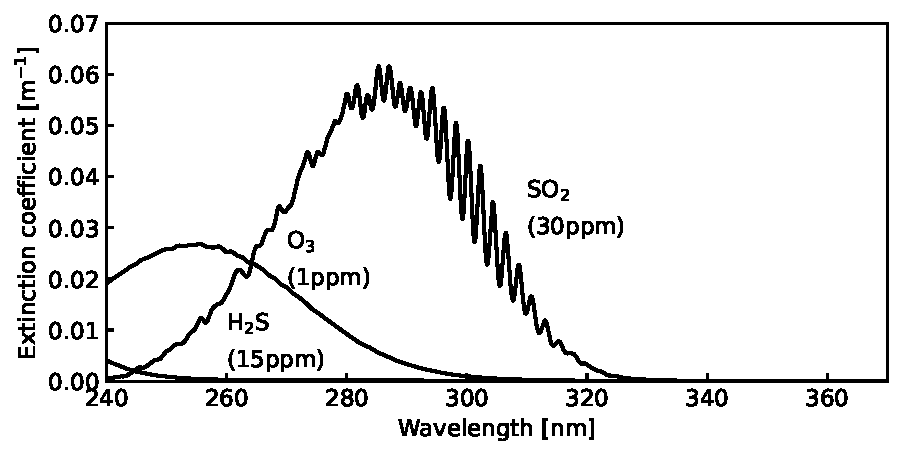
\includegraphics{fig/sim_01_3gases_absorp}
    \caption{\ce{SO2}, \ce{O3}, \ce{H2S}の吸収スペクトル}
    \label{fig:3gases_absorption}
\end{figure}
\noindent
二酸化硫黄は紫外領域に吸収スペクトルを持ち, 
300 nm 付近の波長では吸収が櫛状に増減する特徴を持つ. 
二酸化硫黄測定にラマン DIALを適応する場合, 
\staterr は, これらの吸収スペクトルに依存する. 
改めて, \cref{equ:stat_err}の 
$P$ と $\Delta\subrm{\sigma}{SO2}$はon波長とoff波長に依存し, 
on波長及びoff波長に相当するラマン散乱波長はレーザ波長に依存する. 
したがって, \ce{SO2}測定のためのラマンDIALは, 
火山ガスの吸収スペクトル形状に合わせて,
受信強度と差分吸収が十分に確保できるレーザ波長の最適点が存在する.

\newpage
そして, 受信するon波長とoff波長の構成にも注意する必要がある. 
ラマン散乱におけるレーザ波長\subrm{\lambda}{ls}と
ラマン散乱波長\subrm{\lambda}{ram}, 
ラマンシフト\subrm{\lambda}{shift}の関係は\cref{fig:raman_shift}に示すとおりである. 

\begin{figure}
    \centering
    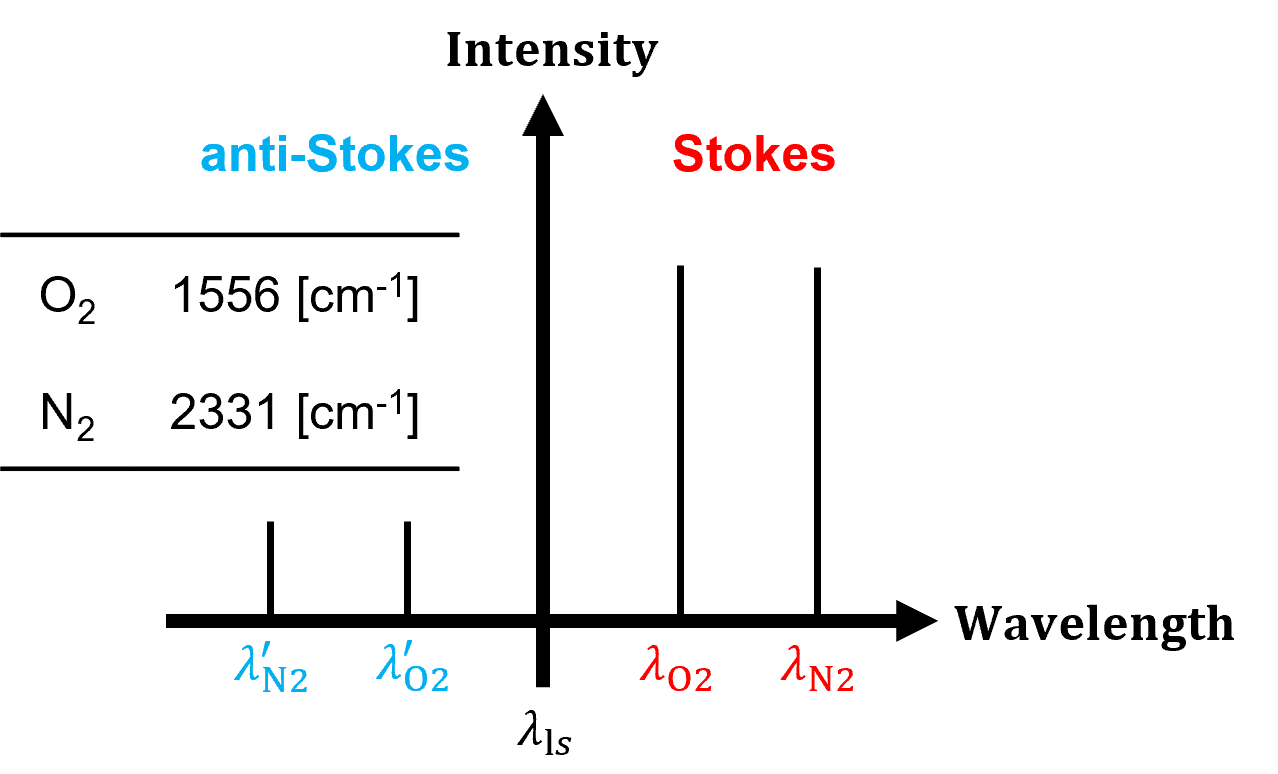
\includegraphics{fig/raman_stokes_Astokes}
    \caption{レーザ波長とラマン散乱波長の関係}
    \label{fig:raman_shift}
\end{figure}

\noindent
酸素分子\ce{O2}によるラマン散乱波長には,
ストークス散乱波長$\subrm{\lambda}{O2}$と
アンチストークス散乱波長$\subrm{\lambda}{O2}'$の2種類が存在し,
窒素分子\ce{N2}についても同様である.
そのため,1つのレーザ波長からラマンDIALの受信波長を構成する場合, 
\ce{O2} および \ce{N2} のストークス・アンチストークス散乱を含む
計 4 つのラマン散乱波長から on 波長および off 波長を選択可能であり,
その組合せは 6 通りとなる.

一般に,アンチストークス散乱はストークス散乱と比較して信号強度が弱く,
ラマンDIALをはじめとしたラマン散乱を利用する測定系では, 
アンチストークス散乱波長は実用上利用されにくい.
そのため,先行研究では Nd:YAG レーザの第 4 高調波である \qty{266}{nm} に対し,
酸素および窒素のストークス散乱波長のみを用いた
ラマンDIAL測定系について検討した\cite{Previous_research}.

しかし, アンチストークス散乱波長が受信波長として利用可能であるとすれば,
従来法の受信波長構成に加えて,新たに 5 つの受信波長構成が検討対象となる.
これら 6 つの受信波長構成は, 
同じレーザ波長でも on 波長および off 波長の波長配置がそれぞれ異なるため,
それに依存する統計誤差 $\staterr$ も異なる.
したがって, その中でも統計誤差が小さい最適な受信波長構成が存在する.

本章では, 6つの受信波長構成で統計誤差を計算し, 比較した結果を示す.
6つの受信波長構成それぞれで最適レーザ波長のときの統計誤差を比較し, 
最も小さいものを最適な受信波長構成とする. 

\newpage
\section{シミュレーション条件}
高度$z$, 波長$\lambda$, ライダー視線距離$R$における大気モデルは以下の通りとした. 
\cref{equ:atmnumber}は大気密度, 
\cref{equ:sigmaray}はレイリー散乱断面積, 
\cref{equ:betamol}は大気分子の後方散乱係数,
\cref{equ:aermodel}エアロゾルモデル, 
\cref{equ:betaaer}はエアロゾルの後方散乱係数, 
\cref{equ:alphamol}は大気分子の消散係数, 
\cref{equ:alphaaer}はエアロゾルの消散係数, 
\cref{equ:alphagas}は光路上の気体の消散係数（$i=1,2,...,N$はN個のガス種）を表す.
\begin{align}
    &N(z)
    =2.60\times10^{25}\exp\left(
        -1.08\times10^{-4}z
    \right)&[\si{m^{-3}}]
    \label{equ:atmnumber}\\
    &\subrm{\sigma}{ray}(\lambda)
    =5.45\times10^{-32}\left(\frac{550}{\lambda}\right)&[\si{m^{2}}]
    \label{equ:sigmaray}\\
    &\subrm{\beta}{mol}(z, \lambda)
    =N(z)\subrm{\sigma}{ray}(\lambda)&[\si{m^{-1}}]
    \label{equ:betamol}\\
    &\subrm{M}{aer}(z, \lambda)
    =36.31\exp(-.78\times10^{-4}\subrm{\beta}{mol}(z))\left(\frac{\lambda}{710}\right)^4
    \label{equ:aermodel}\\
    &\subrm{\beta}{aer}(z, \lambda)
    =\subrm{M}{aer}(z, \lambda)\times\left(\frac{710}{\lambda}\right)&[\si{m^{-1}}]
    \label{equ:betaaer}\\
    &\subrm{\alpha}{mol}=\frac{8\pi}{3}\subrm{\beta}{mol}&[\si{m^{-1}}]
    \label{equ:alphamol}\\
    &\subrm{\alpha}{aer}(z)
    =s\subrm{\beta}{aer}(z)&[\si{m^{-1}}]
    \label{equ:alphaaer}\\
    &\subrm{\alpha}{gas}(z, R, \lambda)
    =\sigma_{i=1}^{N}\subrm{N}{gas}(z, R)\subrm{\sigma}{gas}(\lambda)&[\si{m^{-1}}]
    \label{equ:alphagas}
\end{align}

\cref{fig:gas_setting}に, シミュレーションに用いる火山ガス濃度分布の設定値を示す. 
設定値を決めるにあたって, 三宅島での観測データを参考にした\cite{miyake}.
地表面の火口から二酸化硫黄を含む火山ガスが噴出している環境を想定し, 
高度\qty{1}{km}地点の水平\qty{1}{km}を観測領域に設定した. 
観測領域内の\qty{300}{m}から\qty{700}{m}を火山ガスが濃厚な高濃度区間, 
それ以外を火口から遠い低濃度区間とした. 
気温について, 低濃度区間は\qty{298}{K}, 
高濃度区間は\qty{358}{K}を想定した. 
これは放出される高温の火山ガスがある程度拡散した状況を想定しており, 
気温は用いる吸収断面積のデータセットに反映されている. 
三宅火山は, 近年\ce{SO2}放出量が減少傾向で,
2016年頃から1日あたりの放出量が数十トン以下と少なくなっているが,
三宅空港での監視データでは,
2001年2月から3月末までの2ヶ月間の間に最大で約\qty{11}{ppm}の高濃度が観測されており, 
風による移流の影響を加味すると火口付近はさらに高濃度であると推測される.
そのため, 高濃度区間は二酸化硫黄が\qty{30}{ppm},
硫化水素が\qty{15}{ppm}とし, 
低濃度区間は二酸化硫黄は\qty{0.07}{ppm}
硫化水素は\qty{0.035}{ppm}に設定した. 
オゾンは観測領域全体で一定の\qty{0.005}{ppm}とした. 

\begin{figure}
    \centering
    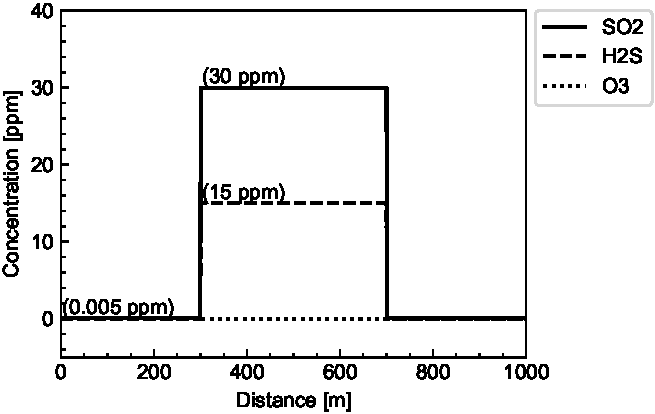
\includegraphics{fig/sim_01_env_LoS}
    \caption{火山ガス濃度分布の設定}
    \label{fig:gas_setting}
\end{figure}

\newpage
\cref{equ:power}及び\cref{equ:stat_err}で用いる
システムパラメータは\cref{tab:sys_params}に示すとおりである.
\begin{table}
    \centering
    \caption{システムパラメータ設定値}
    \label{tab:sys_params}
    \begin{tabular}{lcc}
        \hline
        \hline
        Pluse energy                &$E_0$                      & \qty{10}{mJ} \\
        Laser repetition frequency  &$f$                        & \qty{100}{Hz} \\
        Integration time            &$\subrm{t}{m}$             & \qty{10}{min} \\
        Number of integrations      &$M=f\times \subrm{t}{m}$   & \num{6.0e4}\\
        Receiver telescope diameter &$A$                        & \qty{0.3}{m} \\
        Total optical efficiency    &$q$                        & 0.3 \\
        Detector quantum efficiency &$\eta$                     & 0.3 \\
        Spatial resolution          &$\Delta R$                 & \qty{5}{m} \\
        Dark counts                 &$D$                        & 0\\
        Background light noise      &$B$                        & 0\\
        Detector noise factor       &$F$                        & 1 \\
        \hline
        \hline
    \end{tabular}
\end{table}

\noindent
ラマンDIALによる観測の特徴である時間連続性は積算時間を10 分としており, 
分布観測性は距離分解能を\qty{5}{m}としている. 
すなわち得られる測定データは10分間の時間平均, 
\qty{5}{m}区間の距離平均濃度を意味する. 
また, 本研究全体を通して, 
背景光雑音及びダークカウント, ディテクター雑音指数による影響を
無視した理想条件でシミュレーションした. 

\newpage
\section{受信波長の構成による統計誤差の比較}
\cref{fig:raman_shift}に示したように, 
レーザ波長によって生じるラマン散乱波長は4つあり, 
それらから受信する2波長を選択するとき取り得る構成は6通りとなる. 
それぞれで, \staterr が最小となるレーザ波長を探索し, 
そのときの\staterr の距離特性を比較することで最適な受信波長の構成を決定する.
\cref{fig:6combies_stat}に, 
各受信波長の構成における統計誤差を示す.
\begin{figure}
    \centering
    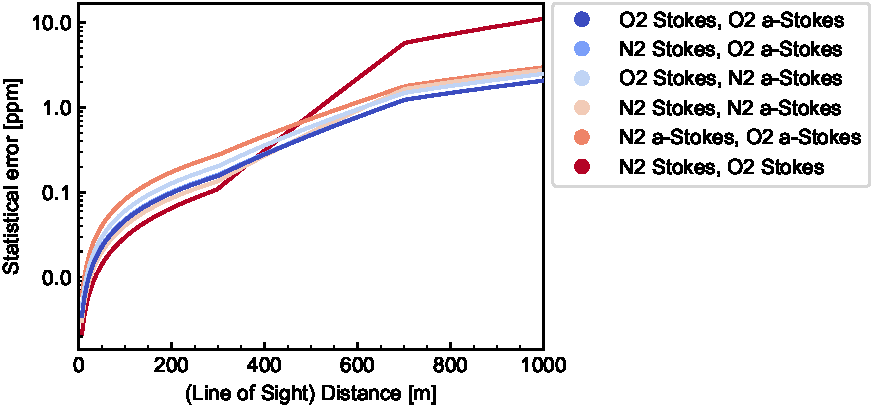
\includegraphics{fig/sim_01_6combies_stat}
    \caption{受信波長の構成による統計誤差の比較}
    \label{fig:6combies_stat}
\end{figure}

\noindent
横軸はライダーの視線距離, 
縦軸は\ce{SO2}測定値に対する統計誤差を表し, 
単位はそれぞれ\unit{m}, \unit{ppm}である. 
それぞれの最適レーザ波長は, 
高濃度区間（\qty{300}{m}から\qty{700}{m}）で最遠方測定点となる
\qty{700}{m}の少し手前を基準に最も統計誤差が最小となるものを選択した.
\ce{N2}ストークス散乱波長と\ce{O2}ストークス散乱波長の構成は, 
視線距離で近傍の低濃度区間では優位であるものの, 
高濃度区間での悪化が激しく, 
観測領域終端では\qty{10}{ppm}を超過した. 
反対に, 
\ce{O2}ストークス散乱波長と\ce{O2}アンチストークス散乱波長の構成は, 
統計誤差の距離悪化が緩やかで, 
その他の構成と比較しても統計誤差が小さかった. 

6つの組み合わせそれぞれの最適レーザ波長とオン波長, オフ波長, 
そして基準点での統計誤差を\cref{tab:6combies_3wlandstaterr}に示す. 
レーザ波長に注目すると, 
\ce{N2}ストークス散乱波長と\ce{O2}ストークス散乱波長の構成は
最適レーザ波長が\qty{240}{nm}で, 
それ以外の構成では\qty{340}{nm}前後となっている.
\cref{fig:3gases_absorption}に示したように, 
波長\qty{240}{nm}付近は\ce{H2S}吸収が存在するため統計誤差が悪化しやすい. 
また, それ以降の波長でも\ce{SO2}, 
\ce{O3}ともに吸収が強くなるため同様に統計誤差が悪化しやすい. 
そのため, 紫外領域となる\ce{340}{nm}付近に最適レーザ波長が集まったと考えられる. 
そして, \staterr に注目すると, 
\ce{SO2}濃度の設定値\qty{30}{ppm}に対して, 
\ce{N2}ストークス散乱波長と\ce{O2}ストークス散乱波長の構成では
\staterr は\qty{5}{ppm}以上であり, 設定値の10\%を超過している. 
しかし, それ以外の構成では1\sim 2\unit{ppm}と数\%であるため, 
これらの組み合わせは今回の条件下において, 
\ce{SO2}測定に適する構成である. 
\begin{table}
    \centering
    \caption{各受信信号構成の最適レーザ波長と受信波長, 統計誤差}
    \label{tab:6combies_3wlandstaterr}
    \begin{tabular}{ccccc}
        \hline
        Combi.  
        & Laser wavelength[\unit{nm}] 
        & \subrm{\lambda}{on}[\unit{nm}] 
        & \subrm{\lambda}{off}[\unit{nm}] 
        & \staterr [\unit{ppm}]\\

        \ce{O2} Stokes, \ce{O2} a-Stokes
        & 334.6
        & 318.0
        & 353.0
        & 1.21\\

        \ce{N2} Stokes, \ce{O2} a-Stokes
        & 334.6
        & 318.0
        & 362.9
        & 1.22\\

        \ce{O2} Stokes, \ce{N2} a-Stokes
        & 343.7
        & 318.2
        & 362.1
        & 1.47\\

        \ce{N2} Stokes, \ce{N2} a-Stokes
        & 338.9
        & 314.1
        & 368.0
        & 1.61\\

        \ce{N2} a-Stokes, \ce{O2} a-Stokes
        & 343.6
        & 318.1
        & 326.1
        & 1.75\\

        \ce{N2} Stokes, \ce{O2} Stokes
        & 240.0
        & 254.2
        & 249.3
        & 5.56\\






        \hline
    \end{tabular}
\end{table}

さらに, 統計誤差の距離特性が劣っていた
\ce{N2}ストークス散乱波長と\ce{O2}ストークス散乱波長の構成と, 
統計誤差の距離特性が優れた
\ce{O2}ストークス散乱波長と\ce{O2}アンチストークス散乱波長の構成に注目する. 
\cref{fig:6combies_stat}に2つの受信波長構成それぞれのレーザ波長, 
on波長及びoff波長における吸収断面積を示す. 
横軸は波長, 縦軸は吸収断面積である. 
\begin{figure}
    \centering
    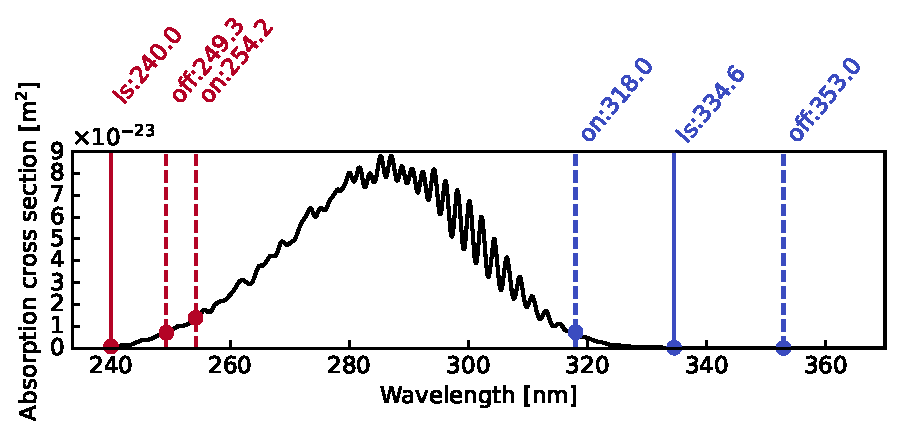
\includegraphics{fig/sim_01_cond_2case}
    \caption{二つの受信波長構成（\ce{N2}ストークス散乱波長と\ce{O2}ストークス散乱波長, 
        \ce{O2}ストークス散乱波長と\ce{O2}アンチストークス散乱波長）における\ce{SO2}吸収断面積}
    \label{fig:cond_wl_combi}
\end{figure}

\noindent
どちらもレーザ波長は山なりの吸収スペクトルから外れており, 
on波長, off波長それぞれの吸収断面積は, 
\ce{N2}ストークス散乱波長と\ce{O2}ストークス散乱波長の構成の方が大きい. 
また, \Delta \subrm{\sigma}{SO2}は, 
\ce{N2}ストークス散乱波長と\ce{O2}ストークス散乱波長の受信構成で\qty{6.83e-24}{m^2}, 
\ce{O2}ストークス散乱波長と\ce{O2}アンチストークス散乱波長の受信構成で\qty{7.22e-24}{m^2}であり, 
僅かに\ce{O2}ストークス散乱波長と\ce{O2}アンチストークス散乱波長の受信構成の方が大きい. 

\cref{fig:cond_power_combi}は, 
\ce{N2}ストークス散乱波長と\ce{O2}ストークス散乱波長の構成と, 
\ce{O2}ストークス散乱波長と\ce{O2}アンチストークス散乱波長の構成における
on波長及びoff波長の信号強度の距離特性であり, 縦軸は受信光子数である. 
\begin{figure}
    \centering
    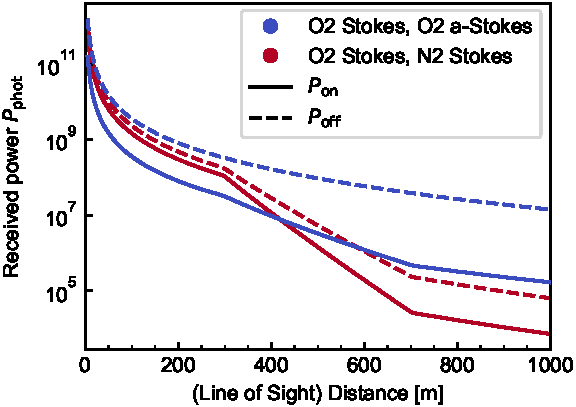
\includegraphics{fig/sim_01_power}
    \caption{
        二つの受信波長構成（\ce{N2}ストークス散乱波長と\ce{O2}ストークス散乱波長, 
        \ce{O2}ストークス散乱波長と\ce{O2}アンチストークス）における受信光子数の距離特性
    }
    \label{fig:cond_power_combi}
\end{figure}

\noindent
赤色で示す\ce{O2}ストークス散乱波長と\ce{N2}ストークス散乱波長の受信波長構成において, 
実線は\ce{N2}ストークス散乱信号（$\subrm{\lambda}{on}=\qty{254.2}{nm}$）, 
点線は\ce{O2}ストークス散乱信号（$\subrm{\lambda}{off}=\qty{249.3}{nm}$）である. 
青色で示す\ce{O2}ストークス散乱波長と\ce{O2}アンチストークス散乱波長の受信波長構成において,
実線は\ce{O2}アンチストークス散乱信号（$\subrm{\lambda}{on}=\qty{318.0}{nm}$）, 
点線は\ce{O2}ストークス散乱信号（$\subrm{\lambda}{off}=\qty{353.0}{nm}$）である. 

\newpage
高濃度の\ce{SO2}による吸収を受ける\qty{300}{m}以前の信号強度を比較すると, 
\cref{equ:power}を解く際に
アンチストークス散乱の信号強度は
ストークス散乱のものに対して1/10となるよう計算したため, 
青実線で示す\ce{O2}アンチストークス散乱は他の3つと比べて小さい.
また, on波長同士では赤色実線で示す\ce{N2}ストークス散乱波長の方が強く, 
off波長同士では青色点線で示す\ce{O2}ストークス散乱波長の方が強い. 
一方で, \qty{700}{m}地点の信号強度を比較すると, 
on波長, off波長どちらも青色で示す
\ce{O2}アンチストークス散乱波長, 
\ce{O2}ストークス散乱波長の方が強い. 
2つの受信構成の$\Delta \subrm{\sigma}{SO2}$は同程度であるため, 
$\subrm{P}{on}, \subrm{P}{off}$が大きい方が
\staterr は小さくなる. 
したがって, 
\ce{O2}アンチストークス散乱波長$\subrm{\lambda}{on}=\qty{318.0}{nm}$の信号強度は
近傍で弱かったものの, 
\ce{SO2}吸収が弱いために信号減衰が小さく, 
遠方での統計誤差に優れた. 

\newpage
\section{ラマンDIALによる二酸化硫黄測定における干渉誤差}
ラマンDIALにおいて測定対象でない物質による吸収は, 
干渉誤差（オフセット誤差）を発生させる. 
火山環境において, 大気や火山ガス中には二酸化硫黄以外にも紫外域に吸収を持つ気体
（オゾンや硫化水素）が存在するため,
それらによる吸収は干渉誤差を引き起こす. 
\cref{equ:contam_err}は干渉要素を補正するための項であり, 
対象気体濃度を算出するためにDIAL方程式を解く際に,
あらかじめ干渉要素の推定値を含めることで 
その影響をある程度補正することが可能である. 
\begin{align}
    \cntmerr
    &= \frac{\Delta \subrm{\alpha}{air}
    +\Sigma^N_{\mathrm{gas}=1}\subrm{n}{gas}\Delta\subrm{\sigma}{gas}}{\Delta \subrm{\sigma}{SO2}}\label{equ:contam_err}
\end{align}
gas=1,2,...,Nは測定時に推定するガス種を表す. 
例えば, オゾンによる干渉を補正したい場合, 
オゾンのおおよその濃度\subrm{n}{O3}を推定し, 
on波長とoff波長における二酸化硫黄, オゾンの差分吸収断面積\subrm{\sigma}{SO2}, \subrm{\sigma}{O3}を
を用意して
\subrm{n}{O3}\times\Delta\subrm{\sigma}{O3}/\Delta\subrm{\sigma}{SO2}
を計算する. これを\cref{equ:n_SO2}から引くことで
補正後の二酸化硫黄濃度の推定値が得られる.
このとき, 推定した濃度が実際の濃度と異なる場合,
干渉誤差が残存することになる.

測定する火山ガス濃度は, 
その火山の熱水系構造や活動状況によって放出量は異なり, 
また, 火口からの距離などによって移流や拡散を伴って濃度は変動する.
そのため, 二酸化硫黄放出が微量であったり, 
それ以外の干渉気体が豊富であったりという
二酸化硫黄の相対量が少ない環境での測定を考えると, 
干渉誤差の影響は無視できないため, 
統計誤差と同様に考慮する必要がある.

\newpage
\cref{fig:6combies_cntm}に各受信波長の構成における干渉誤差を示す. 
横軸はライダーの視線距離, 
縦軸は\ce{SO2}濃度の測定値である. 
\cref{tab:6combies_cntmerr}は低濃度区間にあたる視線距離\qty{100}{m}と
高濃度区間にあたる視線距離\qty{500}{m}における
各受信波長構成の干渉誤差である.

\begin{figure}
    \centering
    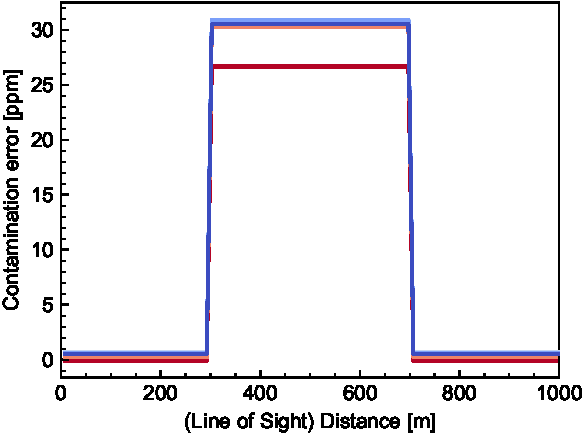
\includegraphics{fig/sim_01_6combies_cntm}
    \caption{受信波長の構成による干渉誤差の比較}
    \label{fig:6combies_cntm}
\end{figure}

\begin{table}
    \centering
    \caption{各受信波長構成の近傍（\qty{100}{m}）及び遠方（\qty{500}{m}）における干渉誤差}
    \label{tab:6combies_cntmerr}
    \begin{tabular}{ccc}
        \hline
        Combi.  
        & \cntmerr(R=100) [\unit{ppm}] 
        & \cntmerr(R=500) [\unit{ppm}] \\

        \ce{O2} Stokes, \ce{O2} a-Stokes
        & 0.47
        & 0.51\\

        \ce{N2} Stokes, \ce{O2} a-Stokes
        & 0.57
        & 0.89\\

        \ce{O2} Stokes, \ce{N2} a-Stokes
        & 0.61
        & 0.93\\

        \ce{N2} Stokes, \ce{N2} a-Stokes
        & 0.48
        & 0.89\\

        \ce{N2} a-Stokes, \ce{O2} a-Stokes
        & 0.14
        & 0.29\\

        \ce{N2} Stokes, \ce{O2} Stokes
        & -0.17
        & -3.32\\
        \hline
    \end{tabular}
\end{table}

\noindent
\ce{N2}ストークス散乱波長と\ce{O2}ストークス散乱波長の構成での
高濃度区間の干渉誤差が\qty{-3.32}{ppm}と最も大きく, 
それ以外の受信波長構成では, 
\qty{1}{ppm}にとどまる結果となった. 
\ce{N2}ストークス散乱波長と\ce{O2}ストークス散乱波長の構成で
干渉誤差が大きくなった理由として, 
統計誤差が他の受信波長構成より大きくなったことと同様に, 
用いる波長が二酸化硫黄やオゾンの吸収が比較的大きい\qty{240}{nm}前後に位置するからだと考えられる. 

\newpage
\section{最適なレーザ波長, 受信波長構成}
本章の結論として, 
統計誤差から決定したレーザ波長及び受信波長構成について, 
レーザ波長は\qty{334.6}{nm}を用いて, 
on波長を\ce{O2}アンチストークス散乱波長の\qty{318.0}{nm} 
off波長を\ce{O2}ストークス散乱波長の\qty{353.0}{nm}とする場合が
最も二酸化硫黄測定に最適なラマンDIALの仕様であると明らかになった.  
統計誤差に影響するレーザ波長, ラマン散乱波長における吸収が従来法より弱く, 
差分吸収断面積が同程度だったことで優位となり, 
結果として, 信号強度が微弱なアンチストークス散乱も, 
波長選択によって十分に選択可能であることが示された. 

この仕様における干渉誤差は, 
今回の条件下の観測領域全体で\ce{0.5}{ppm}前後であり, 
補正なしでも十分に無視できる.
% \begin{figure}[htbp]
%     \centering
%     \begin{subfigure}[b]{0.49\linewidth}
%         \centering
%         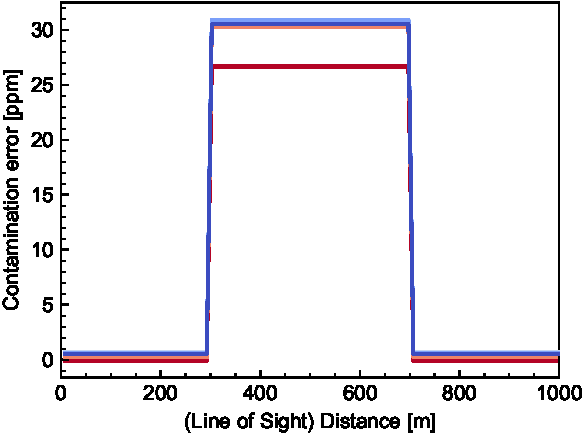
\includegraphics[scale=0.5]{fig/sim_01_6combies_cntm.pdf}
%         \caption{干渉誤差}
%         \label{fig:left}
%     \end{subfigure}
%     \hfill
%     \begin{subfigure}[b]{0.49\linewidth}
%         \centering
%         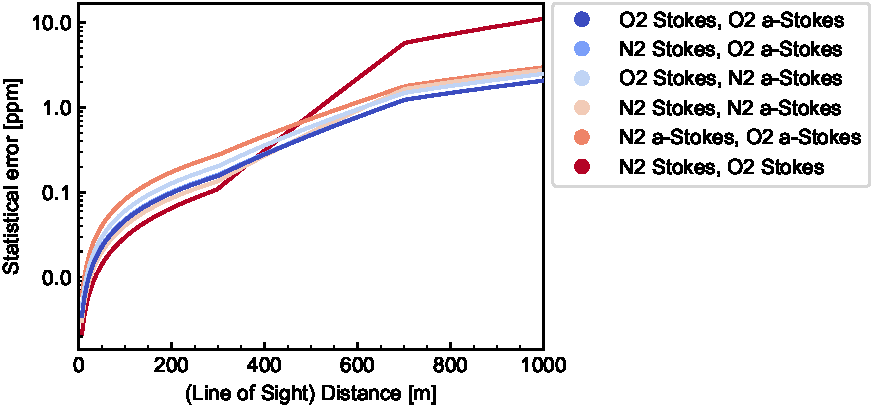
\includegraphics[scale=0.5]{fig/sim_01_6combies_stat.pdf}
%         \caption{統計誤差}
%         \label{fig:right}
%     \end{subfigure}
%     \caption{受信波長の構成による(a)干渉誤差, (b)統計誤差の比較}
%     \label{fig:two_side_by_side}
% \end{figure}
